\part{Lecture 06: \texorpdfstring{$n$-Step}{n-Step} Bootstrapping}
\title[RL Lecture 06]{Lecture 06: \texorpdfstring{$n$-Step}{n-Step} Bootstrapping}  
\date{}  
\frame{\titlepage} 

%%%%%%%%%%%%%%%%%%%%%%%%%%%%%%%%%%%%%%%%%%%%%%%%%%%%%%%%%%%%%
%% Lets Unify MC and One-Step TD Learning %%
%%%%%%%%%%%%%%%%%%%%%%%%%%%%%%%%%%%%%%%%%%%%%%%%%%%%%%%%%%%%%
\frame{\frametitle{Lets Unify MC and One-Step TD Learning}
\begin{figure}		
	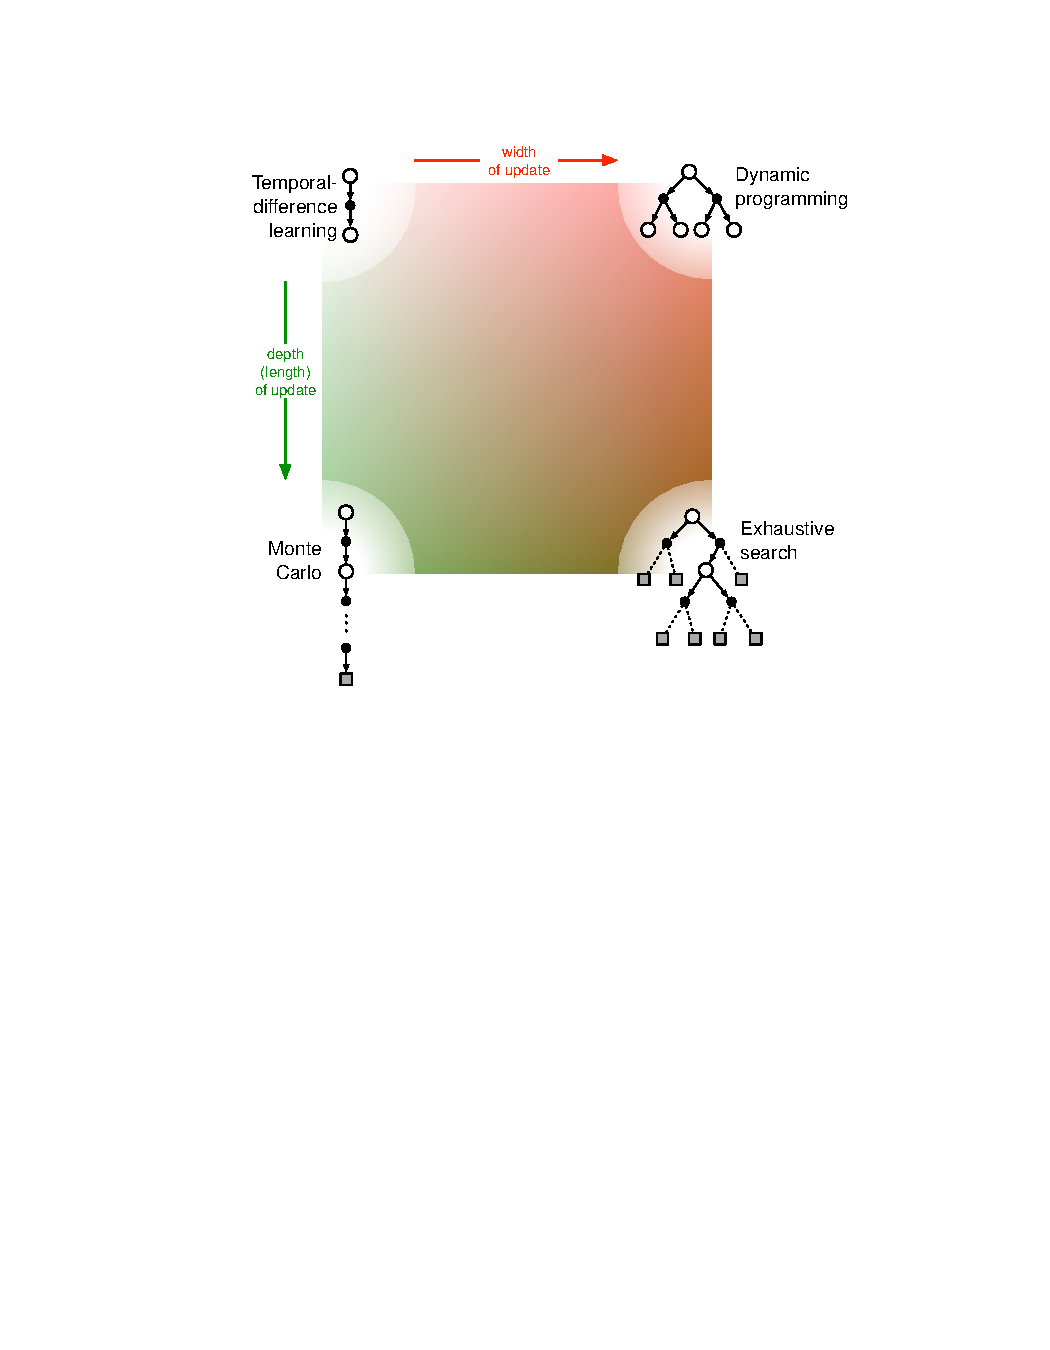
\includegraphics[width=7cm]{fig/lec06/Compare_RL_Methods_Update.pdf}
	\caption{MC and TD are the 'extreme options' in terms of the update's depth: what about intermediate solutions? (source: R. Sutton and G. Barto, Reinforcement learning: an introduction, 2018, \href{https://creativecommons.org/licenses/by-nc-nd/2.0/}{CC BY-NC-ND 2.0})}
	\label{fig:Compare_RL_Methods_Update_lec06}
\end{figure}
}

%%%%%%%%%%%%%%%%%%%%%%%%%%%%%%%%%%%%%%%%%%%%%%%%%%%%%%%%%%%%%%%%%%
\section{\texorpdfstring{$n$-Step}{n-Step} TD Prediction} 
%%%%%%%%%%%%%%%%%%%%%%%%%%%%%%%%%%%%%%%%%%%%%%%%%%%%%%%%%%%%%%%%%%
\begin{frame}
\frametitle{Table of Contents}
\tableofcontents
\end{frame}

%%%%%%%%%%%%%%%%%%%%%%%%%%%%%%%%%%%%%%%%%%%%%%%%%%%%%%%%%%%%%
%% n-Step Bootstrapping Idea %%
%%%%%%%%%%%%%%%%%%%%%%%%%%%%%%%%%%%%%%%%%%%%%%%%%%%%%%%%%%%%%
\frame{\frametitle{$n$-Step Bootstrapping Idea}
\begin{columns}[t,onlytextwidth]
\begin{column}{0.6\textwidth}
\begin{minipage}[c]{\linewidth}
	\begin{figure}		
	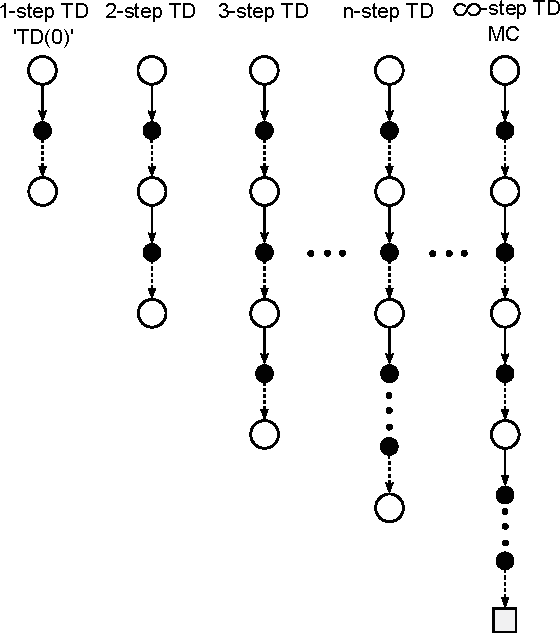
\includegraphics[height=6.25cm]{fig/lec06/Back_Up_n_Step_Methods.pdf}
	\caption{Different backup diagrams of $n$-step state-value prediction methods}
	\label{fig:Back_Up_n_Step_Methods}
\end{figure}
\end{minipage}
\end{column}
\hfill
\begin{column}{0.38\textwidth}
\begin{minipage}[c]{\linewidth}
	\begin{itemize}
		\item $n$-step update: consider $n$ rewards plus estimated value $n$-steps later (bootstrapping).\pause
		\item Consequence: Estimate update is available only after an $n$-step delay.\pause
		\item TD(0) and MC are special cases included in $n$-step prediction.
	\end{itemize}
\end{minipage}
\end{column}
\end{columns}
}

%%%%%%%%%%%%%%%%%%%%%%%%%%%%%%%%%%%%%%%%%%%%%%%%%%%%%%%%%%%%%
%% Formal Notation (1) %%
%%%%%%%%%%%%%%%%%%%%%%%%%%%%%%%%%%%%%%%%%%%%%%%%%%%%%%%%%%%%%
\frame{\frametitle{Formal Notation (1)}
Recap the \hl{update targets} for the incremental prediction methods \eqref{eq:inc_impl_MC_pred_non_stat}:
\begin{itemize}
	\item Monte Carlo: Builds on the complete sampled return series
	\begin{equation}
		g_{k:T} = r_{k+1}+\gamma r_{k+2}+\gamma^2 r_{k+3}+\cdots+\gamma^{T-k-1}r_T .
	\end{equation}
	\begin{itemize}
		\item $g_{k:T}$ denotes that all steps until termination at $T$ are considered to derive an estimate target adressing step $k$.
	\end{itemize}\pause
	\vspace{0.5cm}
	\item TD(0): Utilizes a one-step bootstrapped return
	\begin{equation}
		g_{k:k+1} = r_{k+1}+\gamma \hat{v}_{k}(x_{k+1}) .
	\end{equation}
	\begin{itemize}
		\item For TD(0), $g_{k:k+1}$ highlights that only one future sampled reward step is considered before bootstrapping.
		\item $\hat{v}_{k}$ is an estimate of $v_\pi$ at time step k.
	\end{itemize}
\end{itemize}
}

%%%%%%%%%%%%%%%%%%%%%%%%%%%%%%%%%%%%%%%%%%%%%%%%%%%%%%%%%%%%%
%% Formal Notation (1) %%
%%%%%%%%%%%%%%%%%%%%%%%%%%%%%%%%%%%%%%%%%%%%%%%%%%%%%%%%%%%%%
\frame{\frametitle{Formal Notation (2)}
\begin{block}{$n$-step state-value prediction target}
Now, the target is generalized to an arbitrary $n$-step target:
\begin{equation}
		g_{k:k+n} = r_{k+1}+\gamma r_{k+2}+\cdots+\gamma^{n-1} r_{k+n}+\gamma^{n} \hat{v}_{k+n-1}(x_{k+n}) .
\end{equation}
\end{block}\pause
\begin{itemize}
	\item Approximation of full return series truncated after $n$-steps.
	\item If $k+n \geq T$ (i.e., $n$-step prediction exceeds termination lookahead), then all missing terms are considered zero.
\end{itemize}\pause
\begin{block}{$n$-step TD}
The state-value estimate using the $n$-step return approximation is
\begin{equation}
	\hat{v}_{k+n}(x_k) = \hat{v}_{k+n-1}(x_k) + \alpha \left[g_{k:k+n} - \hat{v}_{k+n-1}(x_k)\right], \quad 0\leq k < T.
\end{equation}
\end{block}\pause
\begin{itemize}
	\item Delay of $n$-steps before $\hat{v}(x)$ is updated.
	\item Additional auxiliary update steps required at the end of each episode.
\end{itemize}
}

%%%%%%%%%%%%%%%%%%%%%%%%%%%%%%%%%%%%%%%%%%%%%%%%%%%%%%%%%%%%%
%% Convergence %%
%%%%%%%%%%%%%%%%%%%%%%%%%%%%%%%%%%%%%%%%%%%%%%%%%%%%%%%%%%%%%
\frame{\frametitle{Convergence}

\begin{theo}{Error reduction property}{error_reduction_property}
The worst error of the expected $n$-step return is always less than or equal to $\gamma^n$ times the worst error under the estimate $\hat{v}_{k+n-1}$:
\begin{equation}
	\max_x \left|\El{G_{k:k+n}|X_k = x}{\pi} - v_\pi(x)\right| \leq \gamma^n \max_x \left|\hat{v}_{k+n-1}(x) - v_\pi(x)\right| .
\end{equation}
\end{theo}\pause
\begin{itemize}
	\item Assuming an infinite number of steps/episodes and an appropriate step-size control according to \theoref{theo:converge_TD_zero}, $n$-step TD prediction converges to the true value.\pause
	\item In a more practical framework with limited number of steps/episodes:
	\begin{itemize}
		\item Choosing the best $n$-step lookahead horizon is an engineering degree of freedom.
		\item This is highly application-dependent (i.e., no predefined optimum).
		\item Prediction/estimation errors can remain due to limited data.
	\end{itemize}
\end{itemize}
}

%%%%%%%%%%%%%%%%%%%%%%%%%%%%%%%%%%%%%%%%%%%%%%%%%%%%%%%%%%%%%
%% Algorithmic Implementation: $n$-step TD-Based Prediction %%
%%%%%%%%%%%%%%%%%%%%%%%%%%%%%%%%%%%%%%%%%%%%%%%%%%%%%%%%%%%%%
\frame{\frametitle{Algorithmic Implementation: $n$-step TD Prediction}
\setlength{\algomargin}{0.5em}
\begin{algorithm}[H]
\small
\SetKwInput{Input}{input} 
\SetKwInput{Output}{output}
\SetKwInput{Init}{init}
\SetKwInput{Param}{parameter}
\Input{a policy $\pi$ to be evaluated}
\Param{step size $\alpha\in(0,1]$, prediction steps $n\in\mathbb{Z}^+$}
\Init{$\hat{v}(x)\, \forall \, x\in\mathcal{X}$ arbitrary except $v_0(x)=0$ if $x$ is terminal}
 \For{$j=1,\ldots,J$ episodes}{
		initialize and store $x_{0}$\;
		$T\leftarrow\infty$\;
		\Repeat( $k=0, 1, 2, \ldots$){$\tau=T-1$}{
			\If{$k<T$}{
				take action from $\pi(x_k)$, observe and store $x_{k+1}$ and $r_{k+1}$\;
				if $x_{k+1}$ is terminal: $T\leftarrow k+1$\;
				}
			$\tau\leftarrow k-n+1$ ($\tau$ time index for estimate update)\;
			\If{$\tau \geq 0$}{
				$g\leftarrow \sum_{i=\tau+1}^{\min(\tau + n, T)}\gamma^{i-\tau-1} r_i$\;
				if $\tau+n < T$: $g\leftarrow g + \gamma^n \hat{v}(x_{\tau+n})$\;
				$\hat{v}(x_{\tau}) \leftarrow \hat{v}(x_{\tau}) + \alpha\left[g - \hat{v}(x_{\tau})\right]$\;
			}
		}
	}
\caption{$n$-step TD prediction (output is an estimate $\hat{v}_\pi(x)$)}
\label{algo:TD_n_step_pred}
\end{algorithm}
}

%%%%%%%%%%%%%%%%%%%%%%%%%%%%%%%%%%%%%%%%%%%%%%%%%%%%%%%%%%%%%
%% Convergence %%
%%%%%%%%%%%%%%%%%%%%%%%%%%%%%%%%%%%%%%%%%%%%%%%%%%%%%%%%%%%%%
\frame{\frametitle{Example: 19 State Random Walk}
\begin{figure}		
	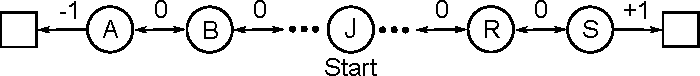
\includegraphics[width=9cm]{fig/lec06/Random_Walk_19_States.pdf}
	\caption{Exemplary random walk Markov reward process (MRP)}
	\label{fig:Random_Walk_19_States}
\end{figure}
\begin{columns}[t,onlytextwidth]
\begin{column}{0.6\textwidth}
\begin{minipage}[c]{\linewidth}
	\begin{figure}		
	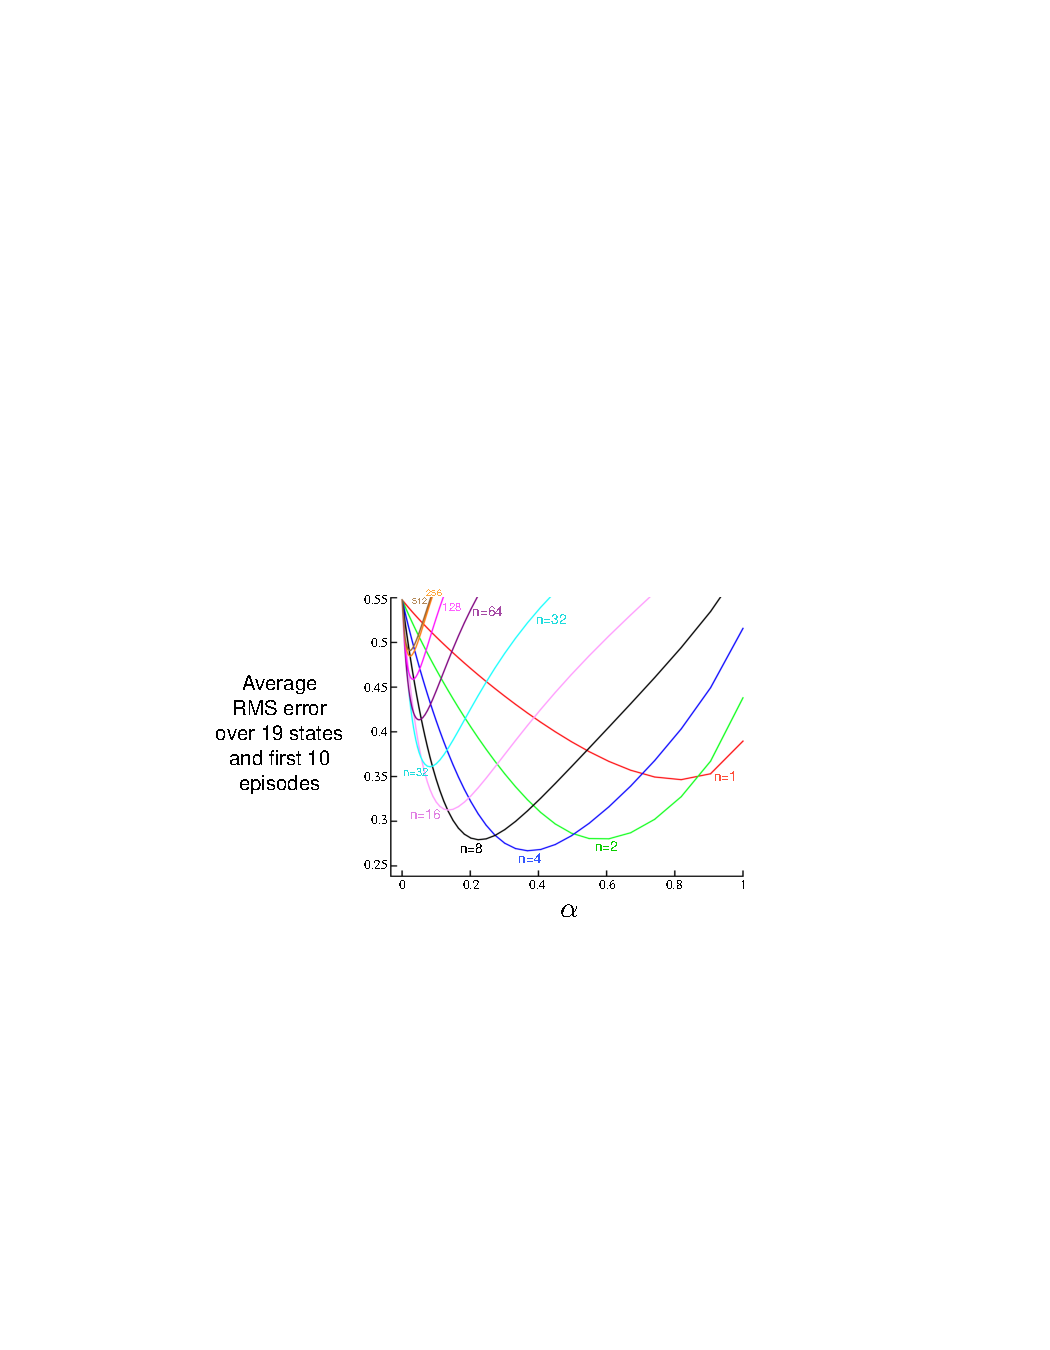
\includegraphics[height=4cm]{fig/lec06/n_Step_TD_Random_Walk.pdf}
	\caption{$n$-step TD performance (source: R. Sutton and G. Barto, Reinforcement learning: an introduction, 2018, \href{https://creativecommons.org/licenses/by-nc-nd/2.0/}{CC BY-NC-ND 2.0})}
	\label{fig:n_Step_TD_Random_Walk}
\end{figure}
\end{minipage}
\end{column}
\hfill
\begin{column}{0.38\textwidth}
\begin{minipage}[c]{\linewidth}
	\begin{itemize}
		\item Early stage performance after only 10 episodes
		\item Averaged over 100 independent runs
		\item Best result here: $n=4, \alpha \approx 0.4$
		\item Picture may change for longer episodes (no generalizable results)
	\end{itemize}
\end{minipage}
\end{column}
\end{columns}
}

%%%%%%%%%%%%%%%%%%%%%%%%%%%%%%%%%%%%%%%%%%%%%%%%%%%%%%%%%%%%%%%%%%
\section{\texorpdfstring{$n$-Step}{n-Step} Sarsa} 
%%%%%%%%%%%%%%%%%%%%%%%%%%%%%%%%%%%%%%%%%%%%%%%%%%%%%%%%%%%%%%%%%%
\begin{frame}
\frametitle{Table of Contents}
\tableofcontents[currentsection]
\end{frame}

%%%%%%%%%%%%%%%%%%%%%%%%%%%%%%%%%%%%%%%%%%%%%%%%%%%%%%%%%%%%%
%% Transfer the $n$-step Approach to State-Action Values (1)%%
%%%%%%%%%%%%%%%%%%%%%%%%%%%%%%%%%%%%%%%%%%%%%%%%%%%%%%%%%%%%%
\frame{\frametitle{Transfer the $n$-step Approach to State-Action Values (1)}
\begin{itemize}
	\item For on-policy control by Sarsa action-value estimates are required. 
	\item Recap the one-step action-value update as required for 'Sarsa(0)':
	\begin{equation}
		\hat{q}(x_k, u_k) \leftarrow \hat{q}(x_k, u_k) + \alpha\left[\underbrace{r_{k+1}+\gamma\hat{q}(x_{k+1}, u_{k+1})}_{\mbox{\footnotesize target }\normalsize g} - \hat{q}(x_k, u_k)\right] .
	\end{equation}
	\end{itemize}\pause
\begin{block}{$n$-step state-action value prediction target}
Analog to $n$-step TD, the state-action value target is rewritten as:
		\begin{equation}
		g_{k:k+n} = r_{k+1}+\gamma r_{k+2}+\cdots+\gamma^{n-1} r_{k+n}+\gamma^{n} \hat{q}_{k+n-1}(x_{k+n}, u_{k+n}) .
\end{equation}
\end{block}\pause
\begin{itemize}
	\item Again, if an episode terminates within the lookahead horizon ($k+n\geq T$) the target is equal to the Monte Carlo update:
	\begin{equation}
		g_{k:k+n}=g_k .
	\end{equation}
\end{itemize}
}


%%%%%%%%%%%%%%%%%%%%%%%%%%%%%%%%%%%%%%%%%%%%%%%%%%%%%%%%%%%%%
%% Transfer $n$-step Update to Action Values (2)%%
%%%%%%%%%%%%%%%%%%%%%%%%%%%%%%%%%%%%%%%%%%%%%%%%%%%%%%%%%%%%%
\frame{\frametitle{Transfer the $n$-step Approach to State-Action Values (2)}
\begin{itemize}
	\item For $n$-step \hl{expected Sarsa}, the update is similar but the state-action value estimate at step $k+n$ becomes the \hl{expected approximate value of $x$} under the target policy valid at time step $k$:
		\begin{equation}
		g_{k:k+n} = r_{k+1}+\gamma r_{k+2}+\cdots+\gamma^{n-1} r_{k+n}+\gamma^{n} \hl{\sum_u \pi(u|x)\hat{q}_k(x,u) }.
		\end{equation}\pause
\item Finally, the modified $n$-step targets can be directly integrated to the state-action value estimate update rule of Sarsa:
\end{itemize}		
\begin{block}{$n$-step Sarsa}
\vspace{-0.4cm}
\begin{equation}
	\hat{q}_{k+n}(x_k,u_k) = \hat{q}_{k+n-1}(x_k,u_k) + \alpha \left[g_{k:k+n} - \hat{q}_{k+n-1}(x_k, u_k)\right], \quad 0\leq k < T.
\end{equation}
\end{block}
}

%%%%%%%%%%%%%%%%%%%%%%%%%%%%%%%%%%%%%%%%%%%%%%%%%%%%%%%%%%%%%
%% $n$-Step Bootstrapping for State-Action Values %%
%%%%%%%%%%%%%%%%%%%%%%%%%%%%%%%%%%%%%%%%%%%%%%%%%%%%%%%%%%%%%
\frame{\frametitle{$n$-Step Bootstrapping for State-Action Values}
\begin{figure}		
	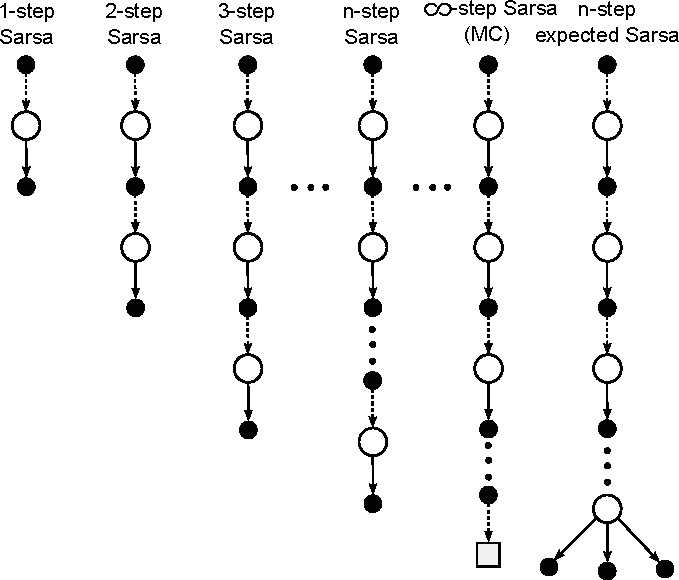
\includegraphics[width=8cm]{fig/lec06/Back_Up_n_Step_Sarsa.pdf}
	\caption{Different backup diagrams of $n$-step state-action value update targets}
	\label{fig:Back_Up_n_Step_Sarsa}
\end{figure}
}

%%%%%%%%%%%%%%%%%%%%%%%%%%%%%%%%%%%%%%%%%%%%%%%%%%%%%%%%%%%%%
%% Algorithmic Implementation: $n$-step Sarsa %%
%%%%%%%%%%%%%%%%%%%%%%%%%%%%%%%%%%%%%%%%%%%%%%%%%%%%%%%%%%%%%
\frame{\frametitle{Algorithmic Implementation: $n$-step Sarsa}
\setlength{\algomargin}{0.5em}
\begin{algorithm}[H]
\footnotesize
\SetKwInput{Input}{input} 
\SetKwInput{Output}{output}
\SetKwInput{Init}{init}
\SetKwInput{Param}{parameter}
%\Output{estimate $\hat{q}_\pi$ or $\hat{q}^*$}
\Param{$\alpha\in(0,1]$, $n\in\mathbb{Z}^+$, $\varepsilon\in\left\{\mathbb{R}|0<\varepsilon<<1\right\}$}
\Init{$\hat{q}(x,u)$ arbitrarily (except terminal states) $\forall \, \left\{x\in\mathcal{X}, u\in\mathcal{U}\right\}$}
\Init{$\pi$ to be $\varepsilon$-greedy with respect to $\hat{q}$ or to a given, fixed policy}
 \For{$j=1,\ldots,J$ episodes}{
		initialize $x_{0}$ and action $u_0 \sim \pi(\cdot | x_0)$ and store them\;
		$T\leftarrow\infty$\;
		\Repeat( $k=0, 1, 2, \ldots$){$\tau=T-1$}{
			\If{$k<T$}{
				take action $u_k$, observe and store $x_{k+1}$ and $r_{k+1}$\;
				\leIf{$x_{k+1}$ is terminal}{$T\leftarrow k+1$}{store $u_{k+1} \sim \pi(\cdot | x_{k+1})$}
			}
			$\tau\leftarrow k-n+1$ ($\tau$ time index for estimate update)\;
			\If{$\tau \geq 0$}{
				$g\leftarrow \sum_{i=\tau+1}^{\min(\tau + n, T)}\gamma^{i-\tau-1} r_i$\;
				if $\tau+n < T$: $g\leftarrow g + \gamma^n \hat{q}(x_{\tau+n}, u_{\tau+n})$\;
				$\hat{q}(x_{\tau},u_{\tau}) \leftarrow \hat{q}(x_{\tau},u_{\tau}) + \alpha\left[g - \hat{q}(x_{\tau}, u_{\tau})\right]$\;
				if $\pi\approx\pi^*$ is being learned, ensure $\pi(\cdot|x_\tau)$ is $\varepsilon$-greedy w.r.t to $\hat{q}$\;
			}
		}
	}
\caption{$n$-step Sarsa (output is an estimate $\hat{q}_\pi$ or $\hat{q}^*$)}
\label{algo:n_step_Sarsa}
\end{algorithm}
}

%%%%%%%%%%%%%%%%%%%%%%%%%%%%%%%%%%%%%%%%%%%%%%%%%%%%%%%%%%%%%
%% Illustration with Grid-World Example %%
%%%%%%%%%%%%%%%%%%%%%%%%%%%%%%%%%%%%%%%%%%%%%%%%%%%%%%%%%%%%%
\frame{\frametitle{Illustration with Grid-World Example}
\begin{figure}		
	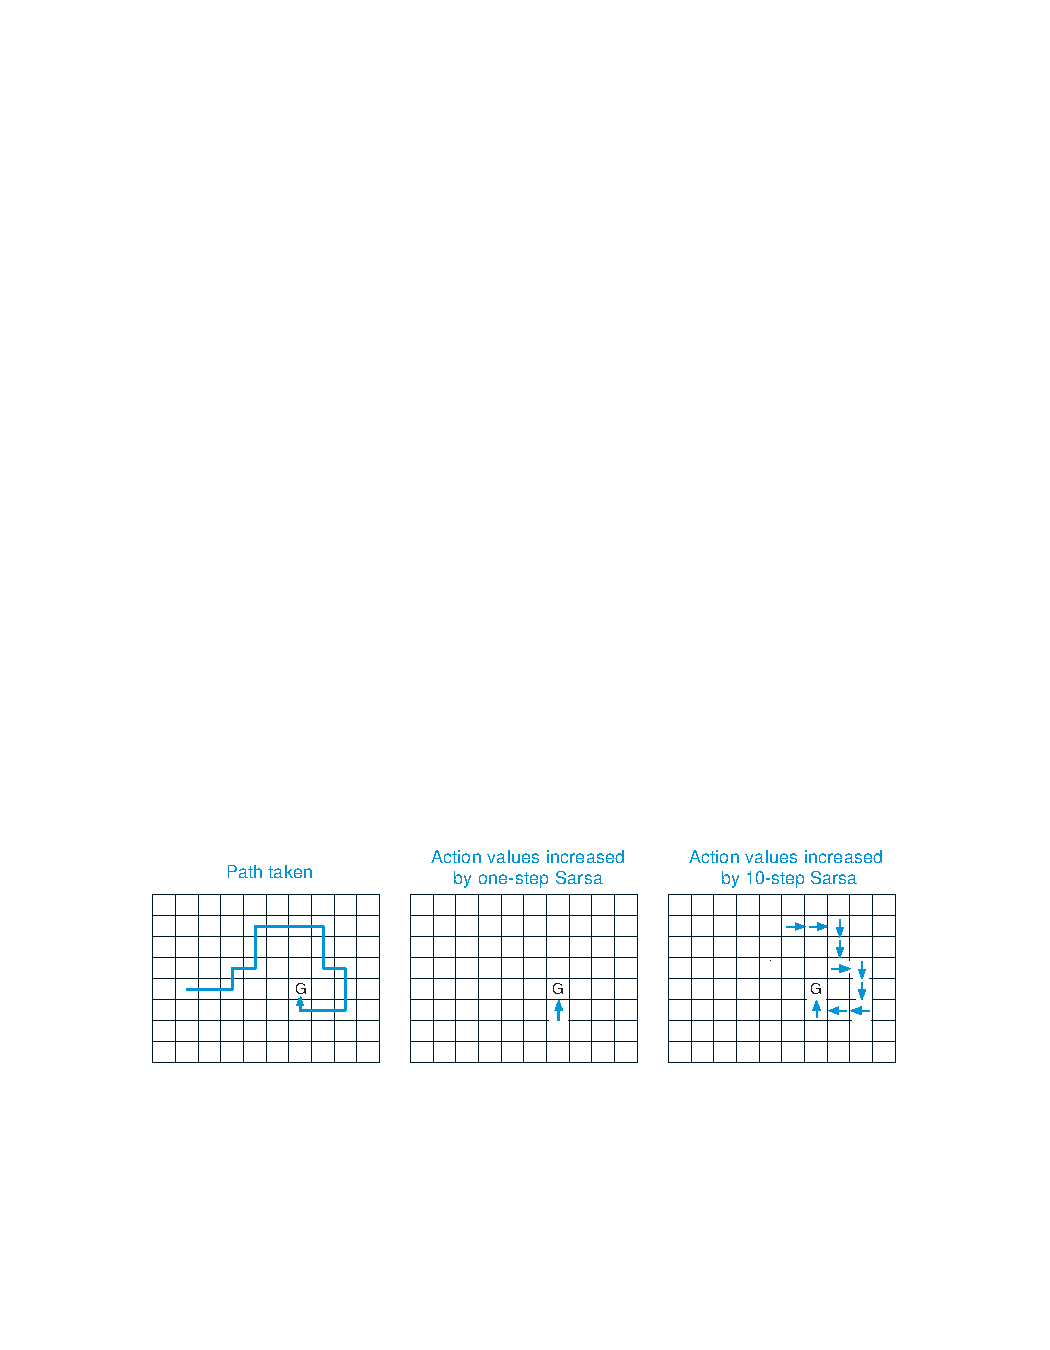
\includegraphics[width=11cm]{fig/lec06/n_step_Sarsa_Grid_World_Example.pdf}
	\caption{Executed updates (highlighted by arrows) for different $n$-step Sarsa implementations during an episode (source: R. Sutton and G. Barto, Reinforcement learning: an introduction, 2018, \href{https://creativecommons.org/licenses/by-nc-nd/2.0/}{CC BY-NC-ND 2.0})}
	\label{fig:n_step_Sarsa_Grid_World_Example}
\end{figure}
\begin{itemize}
	\item For one-step Sarsa, one state-action value is updated.\pause
	\item For ten-step Sarsa, ten state-action values are updated.
	\item In the latter case, much more is learned during one episode.\pause
	\item Nevertheless, a trade-off between the resulting learning delay and the number of updated state-action values remains.
\end{itemize}
}

%%%%%%%%%%%%%%%%%%%%%%%%%%%%%%%%%%%%%%%%%%%%%%%%%%%%%%%%%%%%%%%%%%
\section{\texorpdfstring{$n$-Step}{n-Step} Off-Policy Learning with Importance Sampling} 
%%%%%%%%%%%%%%%%%%%%%%%%%%%%%%%%%%%%%%%%%%%%%%%%%%%%%%%%%%%%%%%%%%
\begin{frame}
\frametitle{Table of Contents}
\tableofcontents[currentsection]
\end{frame}

%%%%%%%%%%%%%%%%%%%%%%%%%%%%%%%%%%%%%%%%%%%%%%%%%%%%%%%%%%%%%
%% Recap on Off-Policy Learning with Importance Sampling%%
%%%%%%%%%%%%%%%%%%%%%%%%%%%%%%%%%%%%%%%%%%%%%%%%%%%%%%%%%%%%%
\frame{\frametitle{Recap on Off-Policy Learning  with Importance Sampling}
Consider two separate policies in order to break the on-policy optimality trade-off:
	\begin{itemize}
		\item \hl{Behavior policy} $b(u|x)$: Explores in order to generate experience.
		\item \hl{Target policy} $\pi(u|x)$: Learns from that experience to become the optimal policy.\pause
		\item Important requirement is \hl{coverage}: Every action taken under $\pi$ must be (at least occasionally) taken under $b$, too. Hence, it follows:
	\begin{equation}
		\pi(u|x) > 0 \Rightarrow b(u|x) > 0 \quad \forall \, \left\{x\in\mathcal{X}, u\in\mathcal{U}\right\} .
	\end{equation}
	\end{itemize}\pause
\begin{block}{Importance sampling ratio (revision from \defref{defi:import_sampl_ratio})}
The relative probability of a trajectory under the target and behavior policy, the importance sampling ratio, from sample step $k$ to $T$ is:
\begin{equation}
	\rho_{k:T}=\frac{\prod_k^{T-1} \pi(u_k|x_{k})p(x_{k+1}|x_{k}, u_{k})}{\prod_k^{T-1} b(u_k|x_{k})p(x_{k+1}|x_{k}, u_{k})}=\frac{\prod_k^{T-1} \pi(u_k|x_{k})}{\prod_k^{T-1} b(u_k|x_{k})} .
\end{equation}
\end{block}
}

%%%%%%%%%%%%%%%%%%%%%%%%%%%%%%%%%%%%%%%%%%%%%%%%%%%%%%%%%%%%%
%% Transfer Importance Sampling to $n$-Step Updates %%
%%%%%%%%%%%%%%%%%%%%%%%%%%%%%%%%%%%%%%%%%%%%%%%%%%%%%%%%%%%%%
\frame{\frametitle{Transfer Importance Sampling to $n$-Step Updates}
For a straightforward \hl{$n$-step off-policy TD-style update}, just weight the update by the importance sampling ratio:
\begin{align}
	\hat{v}_{k+n}(x_k) &= \hat{v}_{k+n-1}(x_k) + \alpha \hl{\rho_{k:k+n-1}}\left[g_{k:k+n} - \hat{v}_{k+n-1}(x_k)\right], \quad 0\leq k < T, \notag \\
										\rho_{k:h}&=	\prod_k^{\min (h,T-1)}\frac{\pi(u_k|x_{k})}{b(u_k|x_{k})} .\label{eq:rho_off_policy_TD}
\end{align}
\begin{itemize}
	\item $\rho_{k:k+n-1}$ is the relative probability under the two polices taking $n$ actions from $u_k$ to $u_{k+n}$.
\end{itemize}\pause
Analog, an \hl{$n$-step off-policy Sarsa-style update} exists:
\begin{equation}
\begin{split}
	\hat{q}_{k+n}(x_k,u_k) &= \hat{q}_{k+n-1}(x_k,u_k) \\&+ \alpha \hl{\rho_{k+1:k+n}}\left[g_{k:k+n} - \hat{q}_{k+n-1}(x_k, u_k)\right], \quad 0\leq k < T.
	\end{split}
\end{equation}
\begin{itemize}
	\item Here, $\rho$ starts and ends one step later compared to the TD case since state-action pairs are updated.
\end{itemize}
}

%%%%%%%%%%%%%%%%%%%%%%%%%%%%%%%%%%%%%%%%%%%%%%%%%%%%%%%%%%%%%
%% Algorithmic Implementation: Off-Policy $n$-step TD Prediction %%
%%%%%%%%%%%%%%%%%%%%%%%%%%%%%%%%%%%%%%%%%%%%%%%%%%%%%%%%%%%%%
\frame{\frametitle{Implementation: Off-Policy $n$-step TD-Based Prediction}
\vspace{-0.15cm}
\setlength{\algomargin}{0.5em}
\begin{algorithm}[H]
\small
\SetKwInput{Input}{input} 
\SetKwInput{Output}{output}
\SetKwInput{Init}{init}
\SetKwInput{Param}{parameter}
\Input{a target policy $\pi$ and a behavior policy $b$ with coverage of $\pi$}
\Param{step size $\alpha\in(0,1]$, prediction steps $n\in\mathbb{Z}^+$}
\Init{$\hat{v}(x)\, \forall \, x\in\mathcal{X}$ arbitrary except $v_0(x)=0$ if $x$ is terminal}
 \For{$j=1,\ldots,J$ episodes}{
		initialize and store $x_{0}$\;
		$T\leftarrow\infty$\;
		\Repeat( $k=0, 1, 2, \ldots$){$\tau=T-1$}{
			\If{$k<T$}{
				take action from $b(x_k)$, observe and store $x_{k+1}$ and $r_{k+1}$\;
				if $x_{k+1}$ is terminal: $T\leftarrow k+1$\;
				}
			$\tau\leftarrow k-n+1$ ($\tau$ time index for estimate update)\;
			\If{$\tau \geq 0$}{
				\hl{$\rho \leftarrow \prod_{i=\tau }^{\min (\tau + n - 2,T-1)}\frac{\pi(u_i|x_{k})}{b(u_i|x_{i})}$}\;
				$g\leftarrow \sum_{i=\tau+1}^{\min(\tau + n, T)}\gamma^{i-\tau-1} r_i$\;
				if $\tau+n < T$: $g\leftarrow g + \gamma^n \hat{v}(x_{\tau+n})$\;
				$\hat{v}(x_{\tau}) \leftarrow \hat{v}(x_{\tau}) + \alpha \hl{\rho}\left[g - \hat{v}(x_{\tau})\right]$\;
			}
		}
	}
\caption{Off-policy $n$-step TD prediction (output is  an estimate $\hat{v}_\pi(x)$)}
\label{algo:TD_n_step_pred_off_policy}
\end{algorithm}
}

%%%%%%%%%%%%%%%%%%%%%%%%%%%%%%%%%%%%%%%%%%%%%%%%%%%%%%%%%%%%%
%% Algorithmic Implementation: Off-Policy $n$-step Sarsa %%
%%%%%%%%%%%%%%%%%%%%%%%%%%%%%%%%%%%%%%%%%%%%%%%%%%%%%%%%%%%%%
\frame{\frametitle{Algorithmic Implementation: Off-Policy $n$-step Sarsa}
\setlength{\algomargin}{0.5em}
\vspace{-0.15cm}
\begin{algorithm}[H]
\footnotesize
\SetKwInput{Input}{input} 
\SetKwInput{Output}{output}
\SetKwInput{Init}{init}
\SetKwInput{Param}{parameter}
\Input{an arbitrary behavior policy $b$ with $b(u|x)>0 \, \forall \, \left\{x\in\mathcal{X}, u\in\mathcal{U}\right\}$}
\Param{$\alpha\in(0,1]$, $n\in\mathbb{Z}^+$, $\varepsilon\in\left\{\mathbb{R}|0<\varepsilon<<1\right\}$}
\Init{$\hat{q}(x,u)$ arbitrarily (except terminal states) $\forall \, \left\{x\in\mathcal{X}, u\in\mathcal{U}\right\}$}
\Init{$\pi$ to be greedy with respect to $\hat{q}$ or to a given, fixed policy}
 \For{$j=1,\ldots,J$ episodes}{
		initialize $x_{0}$ and action $u_0 \sim b(\cdot | x_0)$ and store them\;
		$T\leftarrow\infty$\;
		\Repeat( $k=0, 1, 2, \ldots$){$\tau=T-1$}{
			\If{$k<T$}{
				take action $u_k\sim b(\cdot | x_k)$, observe and store $x_{k+1}$ and $r_{k+1}$\;
				\leIf{$x_{k+1}$ is terminal}{$T\leftarrow k+1$}{store $u_{k+1} \sim b(\cdot | x_{k+1})$}
			}
			$\tau\leftarrow k-n+1$ ($\tau$ time index for estimate update)\;
			\If{$\tau \geq 0$}{
				\hl{$\rho \leftarrow \prod_{i=\tau +1}^{\min (\tau + n -1,T-1)}\frac{\pi(u_i|x_{i})}{b(u_i|x_{i})}$}\;
				$g\leftarrow \sum_{i=\tau+1}^{\min(\tau + n, T)}\gamma^{i-\tau-1} r_i$\;
				if $\tau+n < T$: $g\leftarrow g + \gamma^n \hat{q}(x_{\tau+n}, u_{\tau+n})$\;
				$\hat{q}(x_{\tau},u_{\tau}) \leftarrow \hat{q}(x_{\tau},u_{\tau}) + \alpha \hl{\rho} \left[g - \hat{q}(x_{\tau}, u_{\tau})\right]$\;
				if $\pi\approx\pi^*$ is being learned, ensure $\pi(\cdot|x_\tau)$ is $\varepsilon$-greedy w.r.t to $\hat{q}$\;
			}
		}
	}
\caption{Off-policy $n$-step Sarsa (output is an estimate $\hat{q}_\pi$ or $\hat{q}^*$)}
\label{algo:n_step_Sarsa_off_policy}
\end{algorithm}
}

%%%%%%%%%%%%%%%%%%%%%%%%%%%%%%%%%%%%%%%%%%%%%%%%%%%%%%%%%%%%%%%%%%
\section{\texorpdfstring{$n$-Step}{n-Step} Off-Policy Learning with Tree Backup Approach} 
%%%%%%%%%%%%%%%%%%%%%%%%%%%%%%%%%%%%%%%%%%%%%%%%%%%%%%%%%%%%%%%%%%
\begin{frame}
\frametitle{Table of Contents}
\tableofcontents[currentsection]
\end{frame}

%%%%%%%%%%%%%%%%%%%%%%%%%%%%%%%%%%%%%%%%%%%%%%%%%%%%%%%%%%%%%
%% Off-Policy Learning Without Importance Sampling %%
%%%%%%%%%%%%%%%%%%%%%%%%%%%%%%%%%%%%%%%%%%%%%%%%%%%%%%%%%%%%%
\frame{\frametitle{Off-Policy Learning Without Importance Sampling (1)}
\begin{columns}[t,onlytextwidth]
\begin{column}{0.27\textwidth}
\begin{minipage}[c]{\linewidth}
	\begin{figure}		
	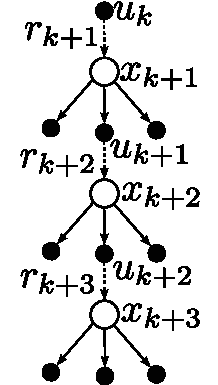
\includegraphics[width=3cm]{fig/lec06/3_step_tree_backup.pdf}
	\caption{3-step tree-backup diagram}
	\label{fig:3_step_tree_backup}
\end{figure}
\end{minipage}
\end{column}
\hfill
\begin{column}{0.72\textwidth}
\begin{minipage}[c]{\linewidth}
	\begin{itemize}
		\item Importance sampling might be tedious and with high variance. Are there alternatives?
		\item For one-step updates, $Q$-learning and expected Sarsa are available as off-policy learning alternatives (see prev. lecture).
		\item Now, tree backups will do the same for $n$-step updates.
	\end{itemize}\pause
	\vspace{1cm}
	General idea:
	\begin{itemize}
		\item Mix $n$-step sampling (middle path on the left) plus bootstrap updates along all not selected actions (dangling nodes hanging off the sides). 
	\end{itemize}
\end{minipage}
\end{column}
\end{columns}
}

%%%%%%%%%%%%%%%%%%%%%%%%%%%%%%%%%%%%%%%%%%%%%%%%%%%%%%%%%%%%%
%% Off-Policy Learning Without Importance Sampling (2) %%
%%%%%%%%%%%%%%%%%%%%%%%%%%%%%%%%%%%%%%%%%%%%%%%%%%%%%%%%%%%%%
\frame{\frametitle{Off-Policy Learning Without Importance Sampling (2)}
\begin{columns}[t,onlytextwidth]
\begin{column}{0.27\textwidth}
\begin{minipage}[c]{\linewidth}
\addtocounter{figure}{-1}
	\begin{figure}		
	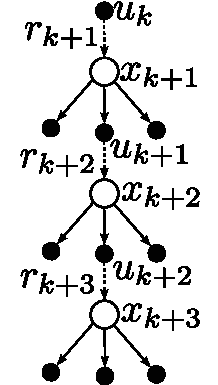
\includegraphics[width=3cm]{fig/lec06/3_step_tree_backup.pdf}
	\caption{3-step tree-backup diagram}
\end{figure}
\end{minipage}
\end{column}
\hfill
\begin{column}{0.72\textwidth}
\begin{minipage}[c]{\linewidth}
	\begin{itemize}
		\item Updates come from the estimated action values of the leaf nodes.
		\item Actions actually taken deliver weights for subsequent nodes proportional to the probability of occurring under $\pi$.
	\end{itemize}\pause
	\vspace{1cm}
	\begin{itemize}
		\item First-level actions contribute to value estimate with weight $\pi(u|x_{k+1})$ .\pause
		\item Second-level actions contribute to value estimate with weight $\pi(u_{k+1}|x_{k+1})\pi(u'|x_{k+2})$ . \pause
		\item Third-level actions contribute to value estimate with weight $\pi(u_{k+2}|x_{k+2})\pi(u_{k+1}|x_{k+1})\pi(u''|x_{k+3})$ . 
	\end{itemize}
\end{minipage}
\end{column}
\end{columns}
}

%%%%%%%%%%%%%%%%%%%%%%%%%%%%%%%%%%%%%%%%%%%%%%%%%%%%%%%%%%%%%
%% Derive Formal Tree-Backup Equations (1)%%
%%%%%%%%%%%%%%%%%%%%%%%%%%%%%%%%%%%%%%%%%%%%%%%%%%%%%%%%%%%%%
\frame{\frametitle{Derive Formal Tree-Backup Equations (1)}
The 1-step tree-backup target is equal to that of expected Sarsa:
		\begin{equation}
		g_{k:k+1} = r_{k+1}+\gamma \sum_{u} \pi(u|x_{k+1}) \hat{q}_k(x_{k+1}, u), \quad k<T-1 .
		\end{equation}\pause
In the 2-step case, the probability of being in $x_{k+1}$ and applying the sampled action $u_{k+1}$ weights the second node (if $k<T-2$):
\begin{equation}
\begin{split}
		g_{k:k+1} &= r_{k+1}+\gamma \sum_{u \neq u_{k+1}} \pi(u|x_{k+1}) \hat{q}_{k+1}(x_{k+1}, u)\\
							&+\gamma \pi(u_{k+1}|x_{k+1})\left(r_{k+2}+\gamma \sum_{u} \pi(u|x_{k+2}) \hat{q}_{k+1}(x_{k+2}, u)\right)\\
							&= r_{k+1}+\gamma \sum_{u \neq u_{k+1}} \pi(u|x_{k+1}) \hat{q}_{k+1}(x_{k+1}, u)+\gamma \pi(u_{k+1}|x_{k+1})g_{k+1:k+2} .
\end{split}
\end{equation}
}

%%%%%%%%%%%%%%%%%%%%%%%%%%%%%%%%%%%%%%%%%%%%%%%%%%%%%%%%%%%%%
%% Derive Formal Tree-Backup Equations (2)%%
%%%%%%%%%%%%%%%%%%%%%%%%%%%%%%%%%%%%%%%%%%%%%%%%%%%%%%%%%%%%%
\frame{\frametitle{Derive Formal Tree-Backup Equations (2)}
Extending the previous scheme delivers a general definition of the tree-backup target in a recursive form:
\begin{block}{$n$-step tree-backup return}
For $k < T-n$ and $n \geq 2$ the $n$-step tree-backup return is:
\begin{equation}
	g_{k:k+n} = r_{k+1}+\gamma \sum_{u \neq u_{k+1}} \pi(u|x_{k+1}) \hat{q}_{k+1}(x_{k+1}, u)+\gamma \pi(u_{k+1}|x_{k+1})g_{k+1:k+n} .
	\label{eq:target_tree_backup}
\end{equation}
\end{block}\pause
\begin{itemize}
	\item Due to recursive formulation, calculation starts at the bottom node.\pause
	\item State-action value update is realized again via the $n$-step Sarsa rule (for $0\leq k < T$):
\begin{equation*}
	\hat{q}_{k+n}(x_k,u_k) = \hat{q}_{k+n-1}(x_k,u_k) + \alpha \left[g_{k:k+n} - \hat{q}_{k+n-1}(x_k, u_k)\right].
\end{equation*}
\end{itemize}
}


%%%%%%%%%%%%%%%%%%%%%%%%%%%%%%%%%%%%%%%%%%%%%%%%%%%%%%%%%%%%%
%% Algorithmic Implementation: $n$-step Tree Backup %%
%%%%%%%%%%%%%%%%%%%%%%%%%%%%%%%%%%%%%%%%%%%%%%%%%%%%%%%%%%%%%
\frame{%\frametitle{Algorithmic Implementation: $n$-step Tree Backup}
\setlength{\algomargin}{0.5em}
\vspace{0.15cm}
\begin{algorithm}[H]
\footnotesize
\SetKwInput{Input}{input} 
\SetKwInput{Output}{output}
\SetKwInput{Init}{init}
\SetKwInput{Param}{parameter}
\Param{$\alpha\in(0,1]$, $n\in\mathbb{Z}^+$}
\Init{$\hat{q}(x,u)$ arbitrarily (except terminal states) $\forall \, \left\{x\in\mathcal{X}, u\in\mathcal{U}\right\}$}
\Init{$\pi$ to be greedy with respect to $\hat{q}$ or to a given, fixed policy}
 \For{$j=1,\ldots,J$ episodes}{
		initialize $x_{0}$ and action $u_0 \sim \pi(\cdot | x_0)$ and store them\;
		$T\leftarrow\infty$\;
		\Repeat( $k=0, 1, 2, \ldots$){$\tau=T-1$}{
			\If{$k<T$}{
				take action $u_k$, observe and store $x_{k+1}$ and $r_{k+1}$\;
				\leIf{$x_{k+1}$ is terminal}{$T\leftarrow k+1$}{store arbitrary $u_{k+1} \sim f(x_{k+1})$ (arbitrary mapping from a behavior policy)}
			}
			$\tau\leftarrow k-n+1$ ($\tau$ time index for estimate update)\;
			\If{$\tau \geq 0$}{
				\leIf{$k+1 \geq T$}{$g \leftarrow r_T$}{ $g\leftarrow r_{k+1} + \gamma \sum_{u} \pi(u|x_{k+1}) \hat{q}(x_{k+1}, u)$}
				\For{$i=\min(k, T-1) : -1 : \tau + 1$}{ $g\leftarrow r_{i} +\gamma \sum_{u \neq u_{i}} \pi(u|x_{i})\hat{q}(x_{i}, u) + \gamma \pi(u_i|x_i) g $}
				$\hat{q}(x_{\tau},u_{\tau}) \leftarrow \hat{q}(x_{\tau},u_{\tau}) + \alpha\left[g - \hat{q}(x_{\tau}, u_{\tau})\right]$\;
				if $\pi\approx\pi^*$ is being learned, ensure $\pi(\cdot|x_\tau)$ is greedy w.r.t to $\hat{q}$\;
			}
		}
	}
\caption{$n$-step tree-backup (output is an estimate $\hat{q}_\pi$ or $\hat{q}^*$)}
\label{algo:n_step_Tree_Backup}
\end{algorithm}
}

%%%%%%%%%%%%%%%%%%%%%%%%%%%%%%%%%%%%%%%%%%%%%%%%%%%%%%%%%%%%%%%%%%
\section{Bringing Everything Together: \texorpdfstring{$n$-Step $Q(\sigma)$}{n-Step Q-Sigma}} 
%%%%%%%%%%%%%%%%%%%%%%%%%%%%%%%%%%%%%%%%%%%%%%%%%%%%%%%%%%%%%%%%%%
\begin{frame}
\frametitle{Table of Contents}
\tableofcontents[currentsection]
\end{frame}

%%%%%%%%%%%%%%%%%%%%%%%%%%%%%%%%%%%%%%%%%%%%%%%%%%%%%%%%%%%%%
%% $n$-Step Bootstrapping for State-Action Values %%
%%%%%%%%%%%%%%%%%%%%%%%%%%%%%%%%%%%%%%%%%%%%%%%%%%%%%%%%%%%%%
\frame{\frametitle{Illustration of the Idea Compared to the Previous Methods}
\begin{figure}		
	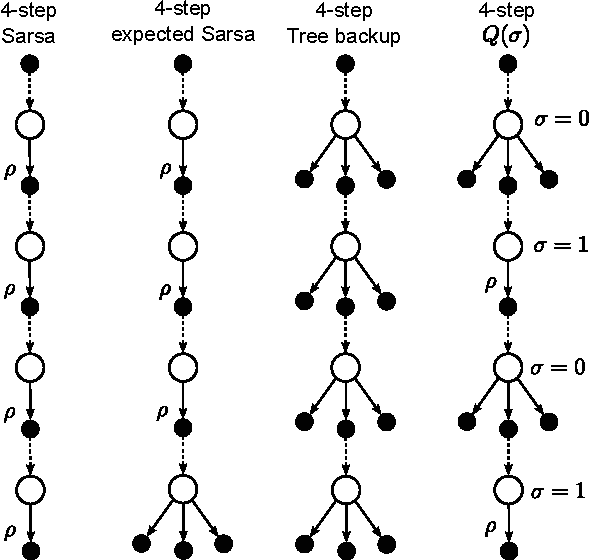
\includegraphics[width=6cm]{fig/lec06/Back_Up_Q_sigma.pdf}
	\caption{The backup diagrams of the previous of $n$-step state-action value updates plus the so-called \hl{$n$-step $Q(\sigma)$} method that unifies
them all (exemplary 4-step case is depicted). \hl{The latter allows for choosing to sample a transition (i.e., $\sigma=1$) or not (i.e., $\sigma=0$) on a state-to-state basis}. A $\rho$ indicates  transitions on which importance sampling is required in the off-policy case.}
	\label{fig:Back_Up_Q_sigma}
\end{figure}
}

%%%%%%%%%%%%%%%%%%%%%%%%%%%%%%%%%%%%%%%%%%%%%%%%%%%%%%%%%%%%%
%% Remarks on $\sigma$ %%
%%%%%%%%%%%%%%%%%%%%%%%%%%%%%%%%%%%%%%%%%%%%%%%%%%%%%%%%%%%%%
\frame{\frametitle{Remarks on $\sigma$}
\begin{itemize}
	\item In each time step $k$, consider a \hl{continuous mixing of sampling and expectation} by $\sigma_k\in [0,1]$. \pause
	\item Special cases are included:
	\begin{itemize}
		\item $\sigma_k=0$: pure expectation,
		\item $\sigma_k=1$: full sampling. \pause
	\end{itemize}
	\item $\sigma_k$ can be set individually for each state either manually or dynamically by superimposed optimization algorithms. \pause
	\item In general, $\sigma_k$ is an important (hyper-)parameter which increases flexibility but also complexity. 
\end{itemize}
}

%%%%%%%%%%%%%%%%%%%%%%%%%%%%%%%%%%%%%%%%%%%%%%%%%%%%%%%%%%%%%
%% $n$-Step $Q(\sigma)$ Target%%
%%%%%%%%%%%%%%%%%%%%%%%%%%%%%%%%%%%%%%%%%%%%%%%%%%%%%%%%%%%%%
\frame{\frametitle{$n$-Step $Q(\sigma)$ Target (1)}
Firstly, we rewrite the $n$-step tree backup \eqref{eq:target_tree_backup}
\begin{equation*}
	g_{k:k+n} = r_{k+1}+\gamma \sum_{u \neq u_{k+1}} \pi(u|x_{k+1}) \hat{q}_{k+1}(x_{k+1}, u)+\gamma \pi(u_{k+1}|x_{k+1})g_{k+1:k+n}
\end{equation*}
using $\overline{v}_k(x_{k})=\sum_u \pi(u|x)\hat{q}_{k}(x_{k}, u)$ for the time horizon $h=k+n$:
\begin{block}{Rewritten $n$-step tree backup target}
\vspace{-0.4cm}
\begin{equation}
\begin{split}
	g_{k:h} &= r_{k+1}+\gamma \overline{v}_{h-1}(x_{k+1})-\gamma \pi(u_{k+1}|x_{k+1})\hat{q}_{h-1}(x_{k+1}, u_{k+1}) \\&+ \gamma \pi(u_{k+1}|x_{k+1})g_{k+1:h}\\
					&= r_{k+1}+\gamma\pi(u_{k+1}|x_{k+1})\left(g_{k+1:h}-\hat{q}_{h-1}(x_{k+1}, u_{k+1})\right)+\gamma \overline{v}_{h-1}(x_{k+1})
\end{split}
\label{eq:n_step_tree_backup_rewritten}
\end{equation}
\end{block}
}

%%%%%%%%%%%%%%%%%%%%%%%%%%%%%%%%%%%%%%%%%%%%%%%%%%%%%%%%%%%%%
%% $n$-Step $Q(\sigma)$ Target%%
%%%%%%%%%%%%%%%%%%%%%%%%%%%%%%%%%%%%%%%%%%%%%%%%%%%%%%%%%%%%%
\frame{\frametitle{$n$-Step $Q(\sigma)$ Target (2)}
Similarly, a recursive formulation for the off-policy importance sampling  target \eqref{eq:rho_off_policy_TD} can be found:
\begin{block}{Rewritten $n$-step importance sampling target}
\vspace{-0.4cm}
\begin{equation}
	g_{k:h} = r_{k+1}+\gamma\rho_{k+1}\left(g_{k+1:h}-\hat{q}_{h-1}(x_{k+1}, u_{k+1})\right)+\gamma \overline{v}_{h-1}(x_{k+1}) .
	\label{eq:n_step_sampling_Q_sigma}
\end{equation}
\end{block}\pause
Inspecting \eqref{eq:n_step_tree_backup_rewritten} for the expectation-based target and \eqref{eq:n_step_sampling_Q_sigma} for the sample-based target, \hl{$Q(\sigma)$ is a linear weighting in terms of the probability $\pi(u_{k+1}|x_{k+1})$ and the importance sampling ratio $\rho_{k+1}$}:
\begin{block}{$n$-step $Q(\sigma)$ target}
\vspace{-0.4cm}
\small
\begin{equation}
\begin{split}
	g_{k:h} &= r_{k+1}\\&+\gamma\hl{\left(\sigma_{k+1}\rho_{k+1}+(1-\sigma_{k+1})\pi(u_{k+1}|x_{k+1})\right)}\left(g_{k+1:h}-\hat{q}_{h-1}(x_{k+1}, u_{k+1})\right)\\&+\gamma \overline{v}_{h-1}(x_{k+1}) .
\end{split}
	\label{eq:n_step_Q_sigma_target}
\end{equation}
\normalsize
\end{block}  
}

%%%%%%%%%%%%%%%%%%%%%%%%%%%%%%%%%%%%%%%%%%%%%%%%%%%%%%%%%%%%%
%% Algorithmic Implementation: $n$-step Tree Backup %%
%%%%%%%%%%%%%%%%%%%%%%%%%%%%%%%%%%%%%%%%%%%%%%%%%%%%%%%%%%%%%
\frame{\frametitle{Algorithmic Implementation: $n$-step $Q(\sigma)$}
\setlength{\algomargin}{0.5em}
\begin{algorithm}[H]
\footnotesize
\SetKwInput{Input}{input} 
\SetKwInput{Output}{output}
\SetKwInput{Init}{init}
\SetKwInput{Param}{parameter}
\Input{a behavior policy $b$ with $b(u|x)>0 \, \forall \, \left\{x\in\mathcal{X}, u\in\mathcal{U}\right\}$}
\Param{$\alpha\in(0,1]$, $n\in\mathbb{Z}^+$, $\varepsilon\in\left\{\mathbb{R}|0<\varepsilon<<1\right\}$, $\sigma_k\in\left\{\mathbb{R}|0\leq\sigma_k \leq 1\right\}$}
\Init{$\hat{q}(x,u)$ arbitrarily (except terminal states) $\forall \, \left\{x\in\mathcal{X}, u\in\mathcal{U}\right\}$}
\Init{$\pi$ to be $\varepsilon$-greedy with respect to $\hat{q}$ or to a given, fixed policy}
\caption{$n$-step $Q(\sigma)$ (output is an estimate $\hat{q}_\pi$ or $\hat{q}^*$)}
\label{algo:n_step_Q_sigma}
\end{algorithm}
\vspace{1cm}
\begin{itemize}
	\item Due to the algorithm's length, the core code is on the next slide.
\end{itemize}
}

%%%%%%%%%%%%%%%%%%%%%%%%%%%%%%%%%%%%%%%%%%%%%%%%%%%%%%%%%%%%%
%% Algorithmic Implementation: $n$-step Tree Backup %%
%%%%%%%%%%%%%%%%%%%%%%%%%%%%%%%%%%%%%%%%%%%%%%%%%%%%%%%%%%%%%
\frame{%\frametitle{Algorithmic Implementation: $n$-step $Q(\sigma)$ (2)}
\setlength{\algomargin}{0.5em}
\begin{algorithm}[H]
\footnotesize
\SetKwInput{Input}{input} 
\SetKwInput{Output}{output}
\SetKwInput{Init}{init}
\SetKwInput{Param}{parameter}
 \For{$j=1,\ldots,J$ episodes}{
		initialize $x_{0}$ and action $u_0 \sim b(\cdot | x_0)$ and store them\;
		$T\leftarrow\infty$\;
		\Repeat( $k=0, 1, 2, \ldots$){$\tau=T-1$}{
			\If{$k<T$}{
				take action $u_k$, observe and store $x_{k+1}$ and $r_{k+1}$\;
				\lIf{$x_{k+1}$ is terminal}{$T\leftarrow k+1$}
				\Else{
					Choose and store $u_{k+1} \sim b(\cdot|x_{k+1})$\;
					Select $\sigma_{k+1}$ and store $\rho_{k+1}=\pi(u_{k+1}|x_{k+1})/b(u_{k+1}|x_{k+1})$\;
				}
			}
			$\tau\leftarrow k-n+1$ ($\tau$ time index for estimate update)\;
			\If{$\tau \geq 0$}{
					$g \leftarrow 0$\;
					\For{$i=\min(k+1, T) : -1 : \tau + 1$}{
						\lIf{i=T}{$g\leftarrow r_T$}
						\Else{
							$\overline{v}\leftarrow \sum_u \pi(u|x_i)\hat{q}(x_i,u)$\;
							$g\leftarrow r_i + \gamma(\sigma_i\rho_i+(1-\sigma_i)\pi(u_i|x_i))(g-\hat{q}(x_i,u_i))+\gamma \overline{v}$\;
						}
				}
				$\hat{q}(x_{\tau},u_{\tau}) \leftarrow \hat{q}(x_{\tau},u_{\tau}) + \alpha\left[g - \hat{q}(x_{\tau}, u_{\tau})\right]$\;
				if $\pi\approx\pi^*$ is being learned, ensure $\pi(\cdot|x_\tau)$ is greedy w.r.t to $\hat{q}$\;
			}
		}
}
\end{algorithm}
}

%%%%%%%%%%%%%%%%%%%%%%%%%%%%%%%%%%%%%%%%%%%%%%%%%%%%%%%%%%%%%
%% Comparison on 19 State Random Walk Example %%
%%%%%%%%%%%%%%%%%%%%%%%%%%%%%%%%%%%%%%%%%%%%%%%%%%%%%%%%%%%%%
\frame{\frametitle{Comparison on 19 State Random Walk Example }
\begin{columns}[t,onlytextwidth]
\begin{column}{0.55\textwidth}
\begin{minipage}[c]{\linewidth}
\addtocounter{figure}{-1}
	\begin{figure}		
	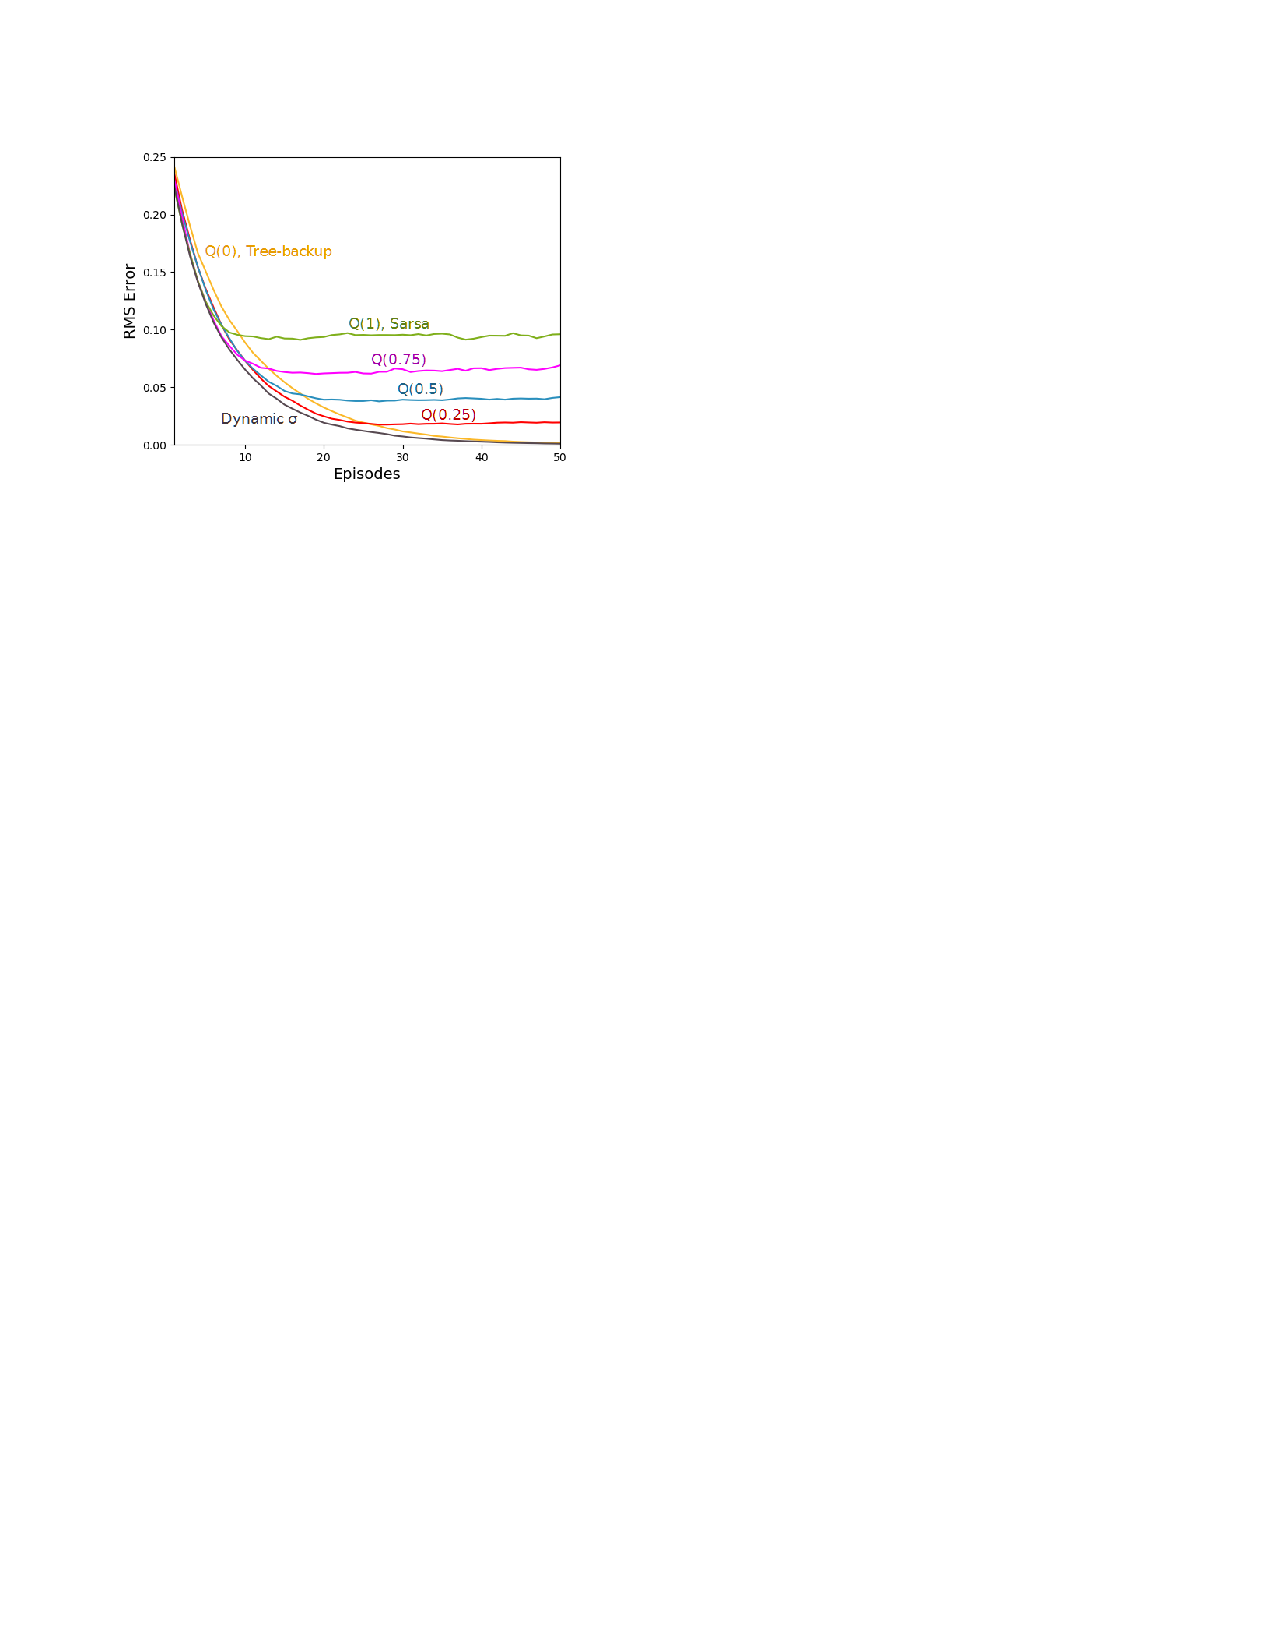
\includegraphics[width=6.25cm]{fig/lec06/Random_Walk_Example_Q_Sigma.pdf}
	\caption{19 state random walk results for different $n$-step algorithms (source:  {De Asis} et al., Multi-step Reinforcement Learning: A Unifying Algorithm, \href{https://arxiv.org/abs/1703.01327}{arXiv:1703.01327}, 2018)}
	\label{fig:Random_Walk_Example_Q_Sigma}
\end{figure}
\end{minipage}
\end{column}
\hfill
\begin{column}{0.44\textwidth}
\begin{minipage}[c]{\linewidth}
	\begin{itemize}
		\item Based on random walk example from \figref{fig:n_Step_TD_Random_Walk}.
		\item $n=3, \alpha=0.4$
		\item Left plot shows RMS error in the value function.
		\item The results are an average of 100 runs. \pause
		\item Dynamic $Q(\sigma)$ starts like Sarsa (i.e., $\sigma = 1$) and shifts towards tree-backup (i.e., $\sigma\approx 0$) by $\sigma_{k+1}=0.95\sigma_k$. \pause
		\item Again: only exemplary application-dependent result.
	\end{itemize}
\end{minipage}
\end{column}
\end{columns}
}

%%%%%%%%%%%%%%%%%%%%%%%%%%%%%%%%%%%%%%%%%%%%%%%%%%%%%%%%%%%%%
%% Summary %%
%%%%%%%%%%%%%%%%%%%%%%%%%%%%%%%%%%%%%%%%%%%%%%%%%%%%%%%%%%%%%
\begin{frame}
\frametitle{Summary: What You've Learned Today}
\begin{itemize}
	\item $n$-step updates allow for an intermediate solution in between temporal difference and Monte Carlo:
	\begin{itemize}
		\item $n=1$: TD as special case,
		\item $n=T$: MC as special case.
	\end{itemize}\pause
	\item The parameter $n$ is a delicate degree of freedom:
	\begin{itemize}
		\item It contains a trade-off between the learning delay and uncertainty reduction when considering more or less steps.
		\item Choosing it is non-trivial and sometimes more art than science.
	\end{itemize}\pause
	\item Tree backups are an alternative for off-policy learning without importance sampling.\pause
	\item $Q(\sigma)$ updates unify sample-based and expectation-based approaches:
	\begin{itemize}
		\item A continuous intermixing of sampling and expectation is possible.
		\item Here, $\sigma_k \in [0,1]$ can be adjusted in every step.
		\item Adds flexibility but obviously also complexity.
		\item Again, optimal parameter choice is not straightforward.
	\end{itemize}
\end{itemize}
\end{frame}

%%%%%%%%%%%%%%%%%%%%%%%%%%%%%%%%%%%%%%%%%%%%%%%%%%%%%%%%%%%%%
%% Final Slide %%
%%%%%%%%%%%%%%%%%%%%%%%%%%%%%%%%%%%%%%%%%%%%%%%%%%%%%%%%%%%%%
\frame{\frametitle{The End for Today}
\vspace{-0.25cm}
\begin{figure}
\hspace*{-0.5cm}

\includegraphics[width=10cm]{fig/lec06/Dilbert.png}
\end{figure}
\vspace{1cm}
\centering
Thanks for your attention and have a nice week!
}